\subsection{Mergeable Data Type}

\begin{figure}[!t]
\centering
\subcaptionbox[] {\small
  When a thread \C{pushes} a new version, it is presumably a semantic
  successor of the version it last \C{pulled} into the heap.
  \label{fig:syntactic-ancestor-1}
} [0.47\columnwidth] {
  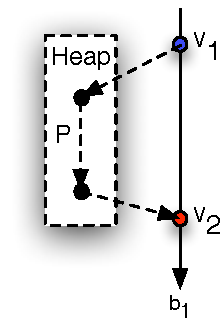
\includegraphics[scale=0.7]{Figures/semantic-ancestor-1}
}
\hfill
\subcaptionbox[] {\small
  Versions created by the \C{merge} operation are syntactic successors
  of merged versions, but need not necessarily be semantic successors.
  \label{fig:syntactic-ancestor-2}
} [0.47\columnwidth] {
  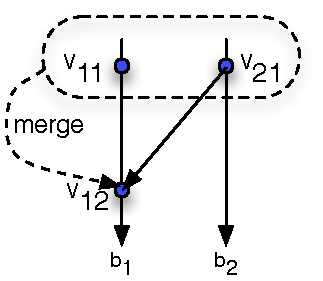
\includegraphics[scale=0.8]{Figures/semantic-ancestor-2}
}
\caption{New versions are created from existing versions either
through \C{push} or \C{merge}.}
\label{fig:syntactic-ancestors}
\end{figure}

We now formally define a mergeable type.  A functional data type
library is a tuple consisting of a type ($t$), and a collection of
functions ($f$, $g$, etc.) of type $t \rightarrow t$ that are
\emph{primitive morphisms}. A morphism ($P$, $Q$, etc.) is either a
primitive morphism, or an associative composition of morphisms ($P
\circ Q \circ R$). An object $B:t$ is called a \emph{semantic
successor} of $A:t$ (conversely, $A$ is called a \emph{semantic
ancestor} of $B$) if and only if there exists a morphism $P$ such that
$P(A) = B$.

The aim of a three-way merge function over a type $t$ is to merge a
pair of semantic successors, $B:t$ and $C:t$, of an object $A:t$, into
another object $D:t$ such that the relationship between the semantic
successors and $D$ satisfies certain conditions. These conditions can
be understood by observing the \rulelabel{E-Pull-Wait} rule of
Fig.~\ref{fig:opsem}, which applies the \C{merge} function to a pair
of concurrent versions ($v_1$ and $v_2$) and their least common
ancestor ($v$). Thus, the only relationship that exists between $v$
and $v_1$, and $v$ and $v_2$ is the syntactic ancestor relationship
that follows from the computation's branching structure. The merge
function, as described above, however assumes that concurrent versions
are semantic successors of their LCA.  It is therefore essential to
maintain coherence between the syntactic and semantic ancestor
relations.

The ways in which syntactic ancestor relationships are created among
versions is captured in Fig.~\ref{fig:syntactic-ancestors}. Whenever an
object is pushed onto the branch, an ancestor relationship is created
between the previous version $v_1$, and the newly created version
$v_2$ (Fig.~\ref{fig:syntactic-ancestor-1}). However, since $v_2$ is
pushed by the thread after reading $v_1$ into the heap, it is
reasonable to assume that $v_2$ is a result of applying a morphism $P$
to $v_1$ (i.e., $\exists P.~v_2 = P(v_1)$).  Hence, $v_1$ is a
semantic ancestor of $v_2$.  Fig.~\ref{fig:syntactic-ancestor-2}
captures another way of establishing an ancestor relationship, namely by
merging branches. Version $v_{21}$ on branch $b_2$ is merged into
$v_{11}$ on $b_1$ to create $v_{12}$ on $b_1$. Versions $v_{11}$ and
\begin{wrapfigure}{l}{.4\textwidth}
\centering
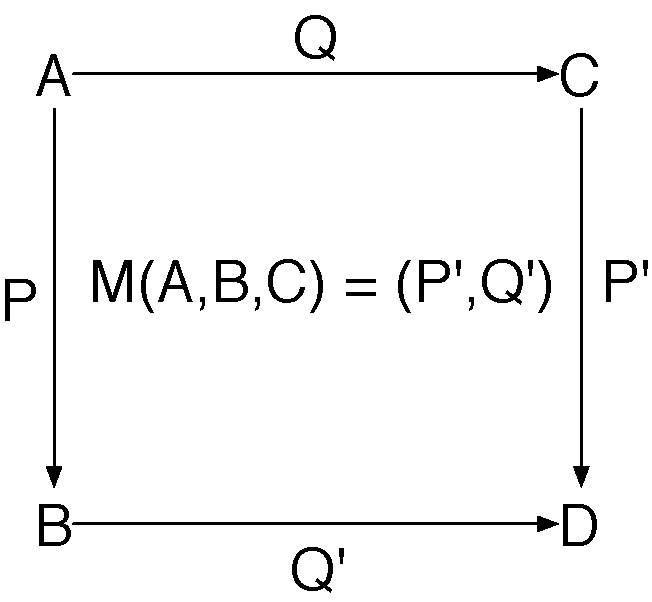
\includegraphics[scale=0.35]{Figures/pushouts}
\caption{Commutative diagram representing the merge operation.}
\label{fig:pushouts}
\end{wrapfigure}
$v_{21}$ are now syntactic ancestors of $v_{12}$, but for them to be
semantic ancestors, the merge function has to enforce the relationship
explicitly. In other words, the result of merging  a pair of
semantic successors, $B$ and $C$, of an $A$, has to be an object $D$
that is a semantic successor of both $B$ and $C$. We now formalize
this intuition to define a mergeable type.
\begin{definition} [\bfseries Mergeable Type]
\label{def:mergeable-type}
A type $t$ is said to be mergeable, if and only if there exists a
function $M$ of type $t \times t \times t \rightarrow (t \rightarrow
t)\times(t \rightarrow t)$ that satisfies the following property:
$\forall (A, B, C\,:\,t).~ (\exists (P,Q\,:\, t \rightarrow t).~ B =
P(A) \conj C = Q(A)) \Rightarrow (\exists (P',Q': t\rightarrow
t).~M(A,B,C) = (P',Q') \conj  Q'(B) = P'(C))$
\end{definition}
Intuitively, a type $t$ is a mergeable type if, whenever there exist
two morphisms $P$ and $Q$ that map $A:t$ to $B:t$ and $C:t$, there
also exists morphisms $P'$ and $Q'$, that map both $B$ and $C$ to
$D:t$. This intuition is expressed visually in
Fig.~\ref{fig:pushouts}.  For a mergeable type $t$, we have the
guarantee that a sequence of values read by a thread from its branch
is sensible, as per the data type semantics:

\begin{theorem} [\bfseries Branch-local consistency]
\label{thm:branch-consistency}
Let $t$ be a mergeable type, and let $H$ be a legal branching history
over values of type $t$. For every pair of values $v_1:t$ and $v_2:t$
along a branch $b$ in $H$, if $\under{H}{v_1 \preceq v_2}$, then there
exists a morphism $P:t\rightarrow t$ such that $v_2 = P(v_1)$.
\end{theorem}

Rather than specifying merge ($M$) in terms of an LCA,
Definition~\ref{def:mergeable-type} specifies $M$ in terms of a pair
of morphisms.  This specification is useful to avoid the expression of certain
nonsensical merge functions, and thus enforce a useful branch-local
consistency property (Theorem~\ref{thm:branch-consistency}). For
instance, consider the counter data type from Sec.~\ref{sec:intro}. A
three-way merge function can be defined to return a constant
regardless of its arguments:
\begin{ocaml}
  let merge lca a b = 0
\end{ocaml}
Such a merge function allows the client to
witness the violation of the branch-local consistency property. For
example, the client may \C{sync} the counter, whose current local
value is $10$, and obtain $0$ as a result, thus witnessing a violation
of counter's monotonicity property. Fortunately,
Def.~\ref{def:mergeable-type} disallows this semantics. It is
impossible to define the function $M$ for the counter data type that
violates the monotonicity invariant, because no counter morphism
violates the invariant. In general, the specification of $M$
guarantees that the merge operation for a type $t$ preserves any
invariants (e.g., balancedness of a tree, sortedness of a list,
non-negativeness of an integer etc) that are preserved by all of $t$'s
morphisms.  The commutativity of the diagram in
Fig.~\ref{fig:pushouts} need not be enforced statically. It can
equally be verified at run-time by checking that the morphisms returned by $M$
map respective concurrent versions to the same value. The
\rulelabel{E-Pull-Wait} rule of the operational semantics
(Fig.~\ref{fig:opsem}) can be extended to this effect:
\begin{smathpar}
\begin{array}{c}
\RULE
{
  t\neq t' \spc
% \under{H}{v' \mbleto v} \spc
% \C{world}(H,t') \semsucceq \C{world}(H,t)\spc 
  v' \not\preceq v \spc
  (P',Q') = M(\C{lca}(H(t),H(t')), v, v') \spc
  Q'(v) = P'(v')
}
{
  (\pull)_t;H(t \mapsto (v,f)::m)(t' \mapsto (v',\_)::\_) ~\stepsto~
  (\pull)_t;H[t \mapsto (v_m,\C{MERGE}\; H(t'))::(v,f)::m]
}
\end{array}
\end{smathpar}

% While the merge function $M$ as specified by
% Def.~\ref{def:mergeable-type} has more verification value, we continue
% to use the three-way merge function \C{merge} in our examples for
% flexibility. 

Def.~\ref{def:mergeable-type} is immediately applicable to simple data
types like counter to explain why they are mergeable. The merge logic
for counter is simple enough that it does not require great effort to
identify the $P$ and $Q$ that lead to the concurrent counter versions,
and transform them into $P'$ and $Q'$ such that the diagram in
Fig.~\ref{fig:pushouts} commutes. For more
\begin{wrapfigure}{l}{.4\textwidth}
\centering
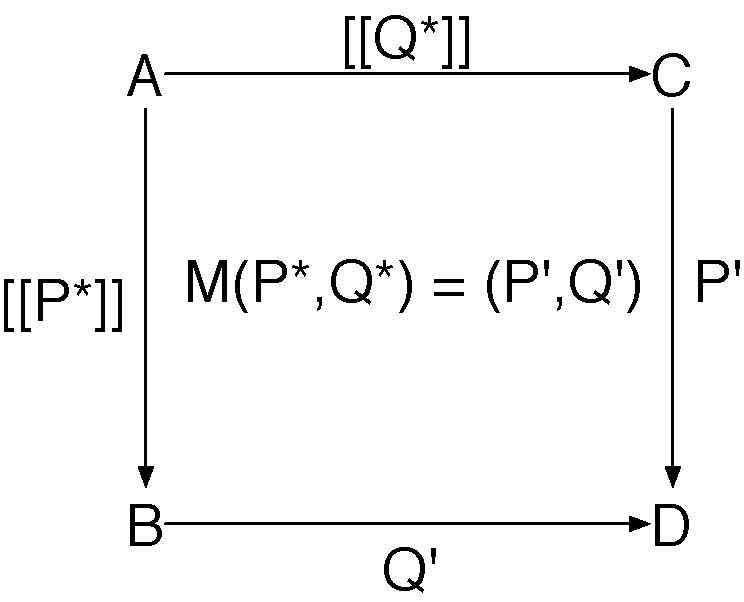
\includegraphics[scale=0.35]{Figures/pushouts-2}
\caption{Commutative diagram for Def.~\ref{def:mergeable-type-2}.}
\label{fig:pushouts-2}
\end{wrapfigure}
sophisticated data types, such as list, this process is more involved,
and may require the programmer to perform non-trivial reasoning. We
now present an alternative definition of a mergeable type that is
stronger than Def.~\ref{def:mergeable-type}, but also serves as a
recipe to build non-trivial merge functions, like that of a list.

\paragraph{Notation} As mentioned earlier, we distinguish between the
named functions defined by a data type library (primitive morphisms),
and their compositions (morphisms). A sequence of primitive morphisms
is written $P^*$ or $Q^*$. The composition of a sequence of primitive
morphisms (written $\denot{P^*}$) is their right-to-left composition,
i.e., $\C{fold\_left}\;(\lambda f.\lambda g. f \circ g)\; id\; P^*$,
where $\C{fold\_left}$ has its usual OCaml type. The length of a
sequence $S$ is written $\length{S}$.

\begin{definition} [\bfseries Mergeable Type]
\label{def:mergeable-type-2}
A type $t$ is said to be mergeable if and only if the following
conditions hold:
\begin{itemize}
  \item There exists a function $W: t \times t \rightarrow (t
  \rightarrow t)^*$ that accepts an object $A:t$ and its
  semantic successor $B:t$, and returns a minimal sequence of
  primitive morphisms $P^*$, whose composition maps $A$ to $B$. That
  is, $W(A,B) = P^*$, where $\denot{P^*}(A) = B$, and there does not
  exist an $R^*$ such that $\denot{R^*}(A) = B$ and $\length{R^*} <
  \length{P^*}$

  \item There exists a function $M: (t \rightarrow t)^*\!\times\!(t
  \rightarrow t)^* \;\rightarrow\; (t \rightarrow t)\!\times\!(t
  \rightarrow t)$ that accepts a pair of minimal sequences of
  primitive morphisms, $P^*$ and $Q^*$, and returns a pair of morphisms,
  $P'$ and $Q'$, such that for any object $A:t$, $(Q' \circ
  \denot{P^*})(A) = (P' \circ \denot{Q^*})(A)$.  
\end{itemize}
The Commutativity diagram of Fig.~\ref{fig:pushouts-2} visualizes this
definition. 
\end{definition}

The definition asserts the existence of two functions for a mergeable
type $t$. First, the function $W$, which (implicitly) computes the
edit distance between an object $A:t$ and its semantic successor
$B:t$.  The sequence of primitive morphisms it returns ($P^*$) is
called an edit sequence. Applying the edit sequence on $A$ produces
$B$ (i.e., $\denot{P^*}(A) = B$). Second, the definition asserts the
existence of a function $M$, which performs an operational
transformation of the primitive morphisms in an edit script. An
operational transformation of a primitive morphism $P$ w.r.t a
morphism $Q$ is another primitive morphism $P'$ such that for any
object $A:t$, $P'$ has the same \emph{effect} on $Q(A)$ as $P$ has on
$A$.

Def.~\ref{def:mergeable-type-2} is immediately applicable to the list
type, and lets us explain why it is a mergeable type.  \C{MList.edit\_seq}
and \C{MList.op\_transform}, respectively, are the evidences for the
existence of $W$ and $M$ functions.
  

